% =========================================================
% Unit Ball Characterisations
% Reference file for: notes-multiple-metrics.tex
% Covers: d1, d2, d_inf on R^2; product std×std; product std×discrete
% =========================================================
\subsubsection{Unit Ball Characterisations}
\label{sec:unit-ball-characterisations}

For a metric space $(X, d)$ and a point $p \in X$, the \emph{open unit ball}
centred at the origin is
\[
B_1(0) \;:=\; \bigl\{\, q \in X : d(0, q) < 1 \,\bigr\}.
\]
Because the unit ball is determined entirely by the metric, different metrics on
the same underlying set $\mathbb{R}^2$ produce geometrically different balls.
The five characterisations below correspond to the five panels in
Figure~\ref{fig:unit-balls-comparison}.

% =========================================================
% 1.  d1
% =========================================================

\begin{tcolorbox}[colback=propbox, colframe=propborder, arc=2pt,
  left=6pt, right=6pt, top=4pt, bottom=4pt,
  title={\small\textbf{Unit Ball: Taxicab Metric $d_1$ on $\mathbb{R}^2$}},
  fonttitle=\small\bfseries]
\begin{definition}[Unit Ball under $d_1$]
\label{def:ball-d1}
Let $d_1(p,q) = |x_1-y_1|+|x_2-y_2|$ on $\mathbb{R}^2$.
The open unit ball centred at the origin is:
\[
B_1^{d_1}(0)
\;=\; \bigl\{\,(x_1,x_2)\in\mathbb{R}^2 :
|x_1| + |x_2| < 1\,\bigr\}.
\]

\medskip
\noindent\textbf{Fully quantified.}
\[
\forall\,(x_1,x_2)\in\mathbb{R}^2:\quad
(x_1,x_2)\in B_1^{d_1}(0)
\;\iff\;
|x_1|+|x_2| < 1.
\]

\medskip
\noindent\textbf{Geometric description.}
A square with vertices at $(\pm 1,0)$ and $(0,\pm 1)$, rotated $45°$
relative to the coordinate axes.
The boundary is the four line segments
$\{(x_1,x_2): |x_1|+|x_2|=1\}$.

\medskip
\noindent\textbf{Boundary formula (four sides).}
\begin{align*}
x_1 \ge 0,\; x_2 \ge 0: &\quad x_1 + x_2 = 1, \\
x_1 \le 0,\; x_2 \ge 0: &\quad -x_1 + x_2 = 1, \\
x_1 \ge 0,\; x_2 \le 0: &\quad x_1 - x_2 = 1, \\
x_1 \le 0,\; x_2 \le 0: &\quad -x_1 - x_2 = 1.
\end{align*}
\end{definition}
\end{tcolorbox}

\begin{remark*}[Extremal points]
The vertices $(\pm 1,0)$ and $(0,\pm 1)$ lie on the boundary.
The corners of the axis-aligned unit square $[\pm1]\times[\pm1]$
do \emph{not}: $d_1\bigl((1,1),(0,0)\bigr) = 2 > 1$.
\end{remark*}

\begin{remark*}[Why ``taxicab'']
$d_1(p,q)$ measures travel distance on a grid where only
horizontal and vertical movement is permitted.
A taxi travelling from $(0,0)$ to $(x_1,x_2)$ must cover
$|x_1|$ blocks east/west and $|x_2|$ blocks north/south,
totalling $|x_1|+|x_2|$ regardless of route.
\end{remark*}

% =========================================================
% 2.  d2
% =========================================================

\begin{tcolorbox}[colback=propbox, colframe=propborder, arc=2pt,
  left=6pt, right=6pt, top=4pt, bottom=4pt,
  title={\small\textbf{Unit Ball: Euclidean Metric $d_2$ on $\mathbb{R}^2$}},
  fonttitle=\small\bfseries]
\begin{definition}[Unit Ball under $d_2$]
\label{def:ball-d2}
Let $d_2(p,q) = \sqrt{(x_1-y_1)^2+(x_2-y_2)^2}$ on $\mathbb{R}^2$.
The open unit ball centred at the origin is:
\[
B_1^{d_2}(0)
\;=\; \bigl\{\,(x_1,x_2)\in\mathbb{R}^2 :
x_1^2 + x_2^2 < 1\,\bigr\}.
\]

\medskip
\noindent\textbf{Fully quantified.}
\[
\forall\,(x_1,x_2)\in\mathbb{R}^2:\quad
(x_1,x_2)\in B_1^{d_2}(0)
\;\iff\;
x_1^2 + x_2^2 < 1.
\]

\medskip
\noindent\textbf{Geometric description.}
The open disc of radius $1$ centred at the origin.
The boundary is the unit circle $\{(x_1,x_2): x_1^2+x_2^2=1\}$.
\end{definition}
\end{tcolorbox}

\begin{remark*}[Rotational symmetry]
$B_1^{d_2}(0)$ is the unique unit ball (among the three standard metrics)
that is invariant under all rotations of $\mathbb{R}^2$:
$d_2(Rp, Rq) = d_2(p,q)$ for every orthogonal matrix $R$.
The $d_1$ and $d_\infty$ balls are only invariant under rotations by
multiples of $90°$.
\end{remark*}

% =========================================================
% 3.  d_inf
% =========================================================

\begin{tcolorbox}[colback=propbox, colframe=propborder, arc=2pt,
  left=6pt, right=6pt, top=4pt, bottom=4pt,
  title={\small\textbf{Unit Ball: Maximum Metric $d_\infty$ on $\mathbb{R}^2$}},
  fonttitle=\small\bfseries]
\begin{definition}[Unit Ball under $d_\infty$]
\label{def:ball-dinf}
Let $d_\infty(p,q) = \max(|x_1-y_1|,|x_2-y_2|)$ on $\mathbb{R}^2$.
The open unit ball centred at the origin is:
\[
B_1^{d_\infty}(0)
\;=\; \bigl\{\,(x_1,x_2)\in\mathbb{R}^2 :
|x_1| < 1 \;\text{ and }\; |x_2| < 1\,\bigr\}.
\]

\medskip
\noindent\textbf{Fully quantified.}
\[
\forall\,(x_1,x_2)\in\mathbb{R}^2:\quad
(x_1,x_2)\in B_1^{d_\infty}(0)
\;\iff\;
\max(|x_1|,|x_2|) < 1
\;\iff\;
(x_1,x_2)\in(-1,1)\times(-1,1).
\]

\medskip
\noindent\textbf{Geometric description.}
The open axis-aligned square $(-1,1)\times(-1,1)$.
The boundary is the perimeter of the unit square
$\{(x_1,x_2): \max(|x_1|,|x_2|)=1\}$.
\end{definition}
\end{tcolorbox}

\begin{remark*}[Equivalence constants]
The three balls are nested for different radii.
Specifically, for all $p \in \mathbb{R}^2$:
\[
B_1^{d_\infty}(0)\;\subseteq\;B_1^{d_2}(0)\;\subseteq\;B_1^{d_1}(0)
\;\subseteq\;B_2^{d_\infty}(0).
\]
This is a geometric restatement of the metric inequalities
$d_\infty \le d_2 \le d_1 \le 2\,d_\infty$.
\end{remark*}

% =========================================================
% 4.  Product std x std
% =========================================================

\begin{tcolorbox}[colback=propbox, colframe=propborder, arc=2pt,
  left=6pt, right=6pt, top=4pt, bottom=4pt,
  title={\small\textbf{Unit Ball: Product Metric (Standard $\times$ Standard)}},
  fonttitle=\small\bfseries]
\begin{definition}[Unit Ball under Standard $\times$ Standard Product]
\label{def:ball-std-std}
Let $d_X = d_Y = |\cdot|$ be the standard metric on $\mathbb{R}$,
and let $d_{\mathrm{sum}} = d_X + d_Y$ be the sum product metric on
$\mathbb{R}\times\mathbb{R}$.
The open unit ball centred at the origin is:
\[
B_1^{d_{\mathrm{sum}}}(0)
\;=\; \bigl\{\,(x_1,x_2)\in\mathbb{R}^2 :
|x_1| + |x_2| < 1\,\bigr\}.
\]

\medskip
\noindent\textbf{Fully quantified.}
\[
\forall\,(x_1,x_2)\in\mathbb{R}^2:\quad
(x_1,x_2)\in B_1^{d_{\mathrm{sum}}}(0)
\;\iff\;
|x_1|+|x_2| < 1.
\]

\medskip
\noindent\textbf{Geometric description.}
Identical to $B_1^{d_1}(0)$: the rotated square with vertices at
$(\pm 1,0)$ and $(0,\pm 1)$.
When both coordinate metrics are the standard metric $|\cdot|$,
the sum product metric \emph{is} the taxicab metric $d_1$.
\end{definition}
\end{tcolorbox}

\begin{remark*}[Why it recovers $d_1$]
$d_{\mathrm{sum}}\bigl((x_1,x_2),(y_1,y_2)\bigr)
= |x_1-y_1| + |x_2-y_2| = d_1\bigl((x_1,x_2),(y_1,y_2)\bigr)$.
The product construction with two standard metric factors is not a
new metric: it is exactly the taxicab metric in disguise.
The product construction becomes genuinely new when the two coordinate
metrics differ.
\end{remark*}

% =========================================================
% 5.  Product std x discrete
% =========================================================

\begin{tcolorbox}[colback=propbox, colframe=propborder, arc=2pt,
  left=6pt, right=6pt, top=4pt, bottom=4pt,
  title={\small\textbf{Unit Ball: Product Metric (Standard $\times$ Discrete)}},
  fonttitle=\small\bfseries]
\begin{definition}[Unit Ball under Standard $\times$ Discrete Product]
\label{def:ball-std-disc}
Let $d_X(x_1,x_2) = |x_1-x_2|$ and
$d_Y(y_1,y_2) = \mathbf{1}_{y_1\neq y_2}$.
The sum product metric on $\mathbb{R}\times\mathbb{R}$ is
$d = d_X + d_Y$.
The open unit ball centred at the origin is:
\[
B_1^{d}(0)
\;=\; \bigl\{\,(x,y)\in\mathbb{R}^2 :
|x| + \mathbf{1}_{y\neq 0} < 1\,\bigr\}.
\]

\medskip
\noindent\textbf{Fully quantified.}
\[
\forall\,(x,y)\in\mathbb{R}^2:\quad
(x,y)\in B_1^{d}(0)
\;\iff\;
\begin{cases}
|x| < 1 & \text{if } y = 0, \\
|x| < 0 & \text{if } y \neq 0.
\end{cases}
\]
Since $|x| < 0$ is impossible, all points with $y \neq 0$ are excluded.
Therefore:
\[
B_1^{d}(0) \;=\; \bigl\{\,(x,0) : |x| < 1\,\bigr\}
\;=\; (-1,1) \times \{0\}.
\]

\medskip
\noindent\textbf{Geometric description.}
The open unit segment on the $x$-axis only.
The ball is a \emph{one-dimensional} subset of $\mathbb{R}^2$:
it has no interior as a subset of the plane.
Every point with $y \neq 0$ lies at distance at least $1$ from the origin.
\end{definition}
\end{tcolorbox}

\begin{remark*}[The ball at a general point]
For an arbitrary centre $(a, b) \in \mathbb{R}^2$, the unit ball is:
\[
B_1^{d}\bigl((a,b)\bigr)
\;=\; \bigl\{\,(x,y) : |x-a| + \mathbf{1}_{y\neq b} < 1\,\bigr\}
\;=\; (a-1,\,a+1) \times \{b\}.
\]
Every unit ball is a horizontal open segment of length $2$ at the same
height as the centre.
Two unit balls at different heights are \emph{disjoint}:
$B_1^d\bigl((a_1, b_1)\bigr) \cap B_1^d\bigl((a_2, b_2)\bigr) = \emptyset$
whenever $b_1 \neq b_2$.
\end{remark*}

\begin{remark*}[No 2-dimensional open sets]
In the standard Euclidean topology on $\mathbb{R}^2$, every open set has
non-empty interior (contains a small disc).
Under $d$, the open sets are unions of horizontal segments --- they are
``thin'' in the vertical direction.
This is a concrete instance of the product metric reflecting the topology
of each coordinate independently:
the discrete metric on $\mathbb{R}$ has only singletons as its connected
components, and the product inherits this vertical rigidity.
\end{remark*}

\begin{remark*}[Balls at radius $r$]
For general $r > 0$, the ball $B_r^{d}\bigl((a,b)\bigr)$ has three regimes:
\[
B_r^{d}\bigl((a,b)\bigr) \;=\;
\begin{cases}
(a-r,\, a+r) \times \{b\}
  & \text{if } 0 < r \le 1, \\[4pt]
\bigl((a-(r-1),\, a+(r-1)) \times \mathbb{R}\bigr)
\cup
\bigl((a-r,\,a+r)\times\{b\}\bigr)
  & \text{if } 1 < r \le 2, \\[4pt]
(a-(r-1),\, a+(r-1)) \times \mathbb{R}
  & \text{if } r > 2.
\end{cases}
\]
At radius $r \le 1$ the ball is a horizontal segment;
at $r > 1$ it begins to include entire vertical fibres
$(a-(r-1), a+(r-1)) \times \{y\}$ for all $y \in \mathbb{R}$,
since any point at horizontal distance less than $r-1$
has total distance less than $(r-1)+1 = r$ from the centre.
At large enough radius the ball grows into an infinite horizontal strip.
\end{remark*}

% ---- wrapper to allow tabular below tikzpicture in standalone ----
\begin{minipage}{18.5cm}

\begin{center}
\small\textbf{Unit balls $B_1(0)$ for five metrics on $\mathbb{R}^2$}
\medskip

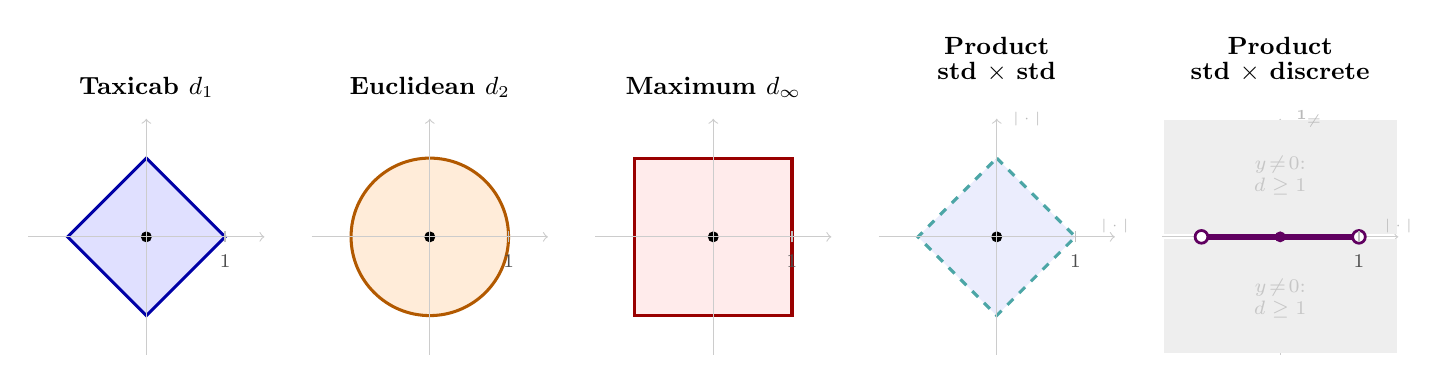
\begin{tikzpicture}[
  dot/.style={circle,fill,inner sep=1.4pt},
  lbl/.style={font=\small},
  sublbl/.style={font=\scriptsize,text=gray!60!black},
]
\def\dx{3.6}
\def\s{1.0}

% ----- Panel 1: d1 taxicab -----
\begin{scope}[shift={(0,0)}]
  \fill[blue!12]   (0,\s)--(\s,0)--(0,-\s)--(-\s,0)--cycle;
  \draw[blue!65!black,line width=1.1pt] (0,\s)--(\s,0)--(0,-\s)--(-\s,0)--cycle;
  \node[dot] at (0,0) {};
  \draw[gray!40,->] (-1.5,0)--(1.5,0);
  \draw[gray!40,->] (0,-1.5)--(0,1.5);
  \draw[gray!50,line width=0.5pt] (\s,-2pt)--(\s,2pt);
  \node[sublbl,anchor=north] at (\s,-3pt) {$1$};
  \node[lbl,font=\small\bfseries,anchor=south] at (0,1.65) {Taxicab $d_1$};
\end{scope}

% ----- Panel 2: d2 Euclidean -----
\begin{scope}[shift={(\dx,0)}]
  \fill[orange!15] (0,0) circle (\s);
  \draw[orange!70!black,line width=1.1pt] (0,0) circle (\s);
  \node[dot] at (0,0) {};
  \draw[gray!40,->] (-1.5,0)--(1.5,0);
  \draw[gray!40,->] (0,-1.5)--(0,1.5);
  \draw[gray!50,line width=0.5pt] (\s,-2pt)--(\s,2pt);
  \node[sublbl,anchor=north] at (\s,-3pt) {$1$};
  \node[lbl,font=\small\bfseries,anchor=south] at (0,1.65) {Euclidean $d_2$};
\end{scope}

% ----- Panel 3: d_inf max/square -----
\begin{scope}[shift={(2*\dx,0)}]
  \fill[red!8]  (-\s,-\s) rectangle (\s,\s);
  \draw[red!60!black,line width=1.1pt] (-\s,-\s) rectangle (\s,\s);
  \node[dot] at (0,0) {};
  \draw[gray!40,->] (-1.5,0)--(1.5,0);
  \draw[gray!40,->] (0,-1.5)--(0,1.5);
  \draw[gray!50,line width=0.5pt] (\s,-2pt)--(\s,2pt);
  \node[sublbl,anchor=north] at (\s,-3pt) {$1$};
  \node[lbl,font=\small\bfseries,anchor=south] at (0,1.65) {Maximum $d_\infty$};
\end{scope}

% ----- Panel 4: product std x std -----
\begin{scope}[shift={(3*\dx,0)}]
  \fill[green!10!blue!8] (0,\s)--(\s,0)--(0,-\s)--(-\s,0)--cycle;
  \draw[green!50!blue!70,line width=1.1pt,dashed]
    (0,\s)--(\s,0)--(0,-\s)--(-\s,0)--cycle;
  \node[dot] at (0,0) {};
  \draw[gray!40,->] (-1.5,0)--(1.5,0);
  \draw[gray!40,->] (0,-1.5)--(0,1.5);
  \draw[gray!50,line width=0.5pt] (\s,-2pt)--(\s,2pt);
  \node[sublbl,anchor=north] at (\s,-3pt) {$1$};
  \node[sublbl,text=gray!55,anchor=south] at (1.5,-0.08) {\tiny$|\cdot|$};
  \node[sublbl,text=gray!55,anchor=west,rotate=0] at (0.08,1.5) {\tiny$|\cdot|$};
  \node[lbl,font=\small\bfseries,anchor=south,align=center] at (0,1.85)
    {Product\\[-2pt]std $\times$ std};
\end{scope}

% ----- Panel 5: product std x discrete -----
\begin{scope}[shift={(4*\dx,0)}]
  \draw[gray!40,->] (-1.5,0)--(1.5,0);
  \draw[gray!40,->] (0,-1.5)--(0,1.5);
  % forbidden band shading
  \fill[gray!13] (-1.48, 0.03) rectangle (1.48, 1.48);
  \fill[gray!13] (-1.48,-1.48) rectangle (1.48,-0.03);
  \node[sublbl,align=center,text=gray!45] at (0, 0.78) {$y\!\neq\!0$:\\$d\ge 1$};
  \node[sublbl,align=center,text=gray!45] at (0,-0.78) {$y\!\neq\!0$:\\$d\ge 1$};
  % unit ball segment
  \draw[violet!75!black,line width=2.4pt] (-\s,0)--(\s,0);
  \draw[violet!75!black,fill=white,line width=1.0pt] (-\s,0) circle (2.3pt);
  \draw[violet!75!black,fill=white,line width=1.0pt] ( \s,0) circle (2.3pt);
  \node[dot,fill=violet!75!black] at (0,0) {};
  \draw[gray!50,line width=0.5pt] (\s,-2pt)--(\s,2pt);
  \node[sublbl,anchor=north] at (\s,-3pt) {$1$};
  \node[sublbl,text=gray!55,anchor=south] at (1.5,-0.08) {\tiny$|\cdot|$};
  \node[sublbl,text=gray!55,anchor=west] at (0.08,1.5) {\tiny$\mathbf{1}_{\neq}$};
  \node[lbl,font=\small\bfseries,anchor=south,align=center] at (0,1.85)
    {Product\\[-2pt]std $\times$ discrete};
\end{scope}

\end{tikzpicture}

\smallskip
\begin{tabular}{@{} l l l @{}}
\toprule
\textbf{Panel} & \textbf{Metric} & \textbf{Unit ball $B_1(0)$} \\
\midrule
Taxicab $d_1$
  & $d_1 = |x_1-y_1|+|x_2-y_2|$
  & Diamond (square rotated $45°$) \\
Euclidean $d_2$
  & $d_2 = \sqrt{(x_1-y_1)^2+(x_2-y_2)^2}$
  & Disc \\
Maximum $d_\infty$
  & $d_\infty = \max(|x_1-y_1|,\,|x_2-y_2|)$
  & Square (axis-aligned) \\
Product std $\times$ std
  & $d = |x_1-x_2|+|y_1-y_2|$
  & Diamond — same as $d_1$ \\
Product std $\times$ discrete
  & $d = |x_1-x_2|+\mathbf{1}_{y_1\neq y_2}$
  & Open segment $\{(x,0):|x|<1\}$ only \\
\bottomrule
\end{tabular}

\smallskip
{\scriptsize\color{gray!60!black}
Panels 1--3: all three standard metrics are equivalent (same open sets, same convergent sequences). \quad
Panel 4: product of two standard metrics recovers $d_1$. \quad
Panel 5: standard $\times$ discrete --- unit ball collapses to a 1-D segment; every off-axis point is at distance $\ge 1$.}

\end{center}
\end{minipage}